\begin{figure}[htbp]
  \centering
  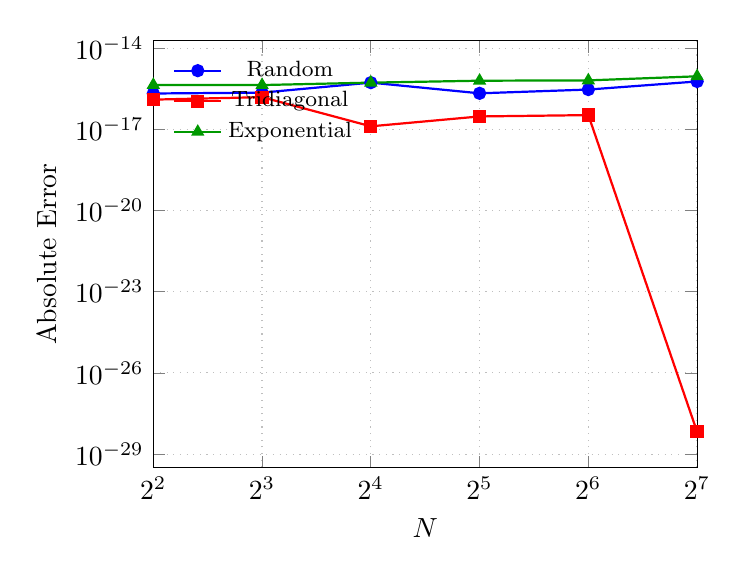
\begin{tikzpicture}
  \begin{axis}[
      width=0.7\linewidth,
      height=7.0cm,
      xmode=log,
      ymode=log,
      log basis x=2,
      xlabel={$N$},
      ylabel={Absolute Error},
      grid=both,
      grid style={dotted},
      minor tick num=0,
      enlarge x limits=false,
      legend style={
          font=\footnotesize,
          draw=none,
          fill=none,
          at={(0.02,0.98)},
          anchor=north west
      }
  ]

  % --- Random Plot ---
  \addplot[blue, thick, mark=*] coordinates {
  (4, 2.113294e-16) (8, 2.271675e-16) (16, 5.327904e-16) (32, 2.145947e-16) (64, 2.956085e-16) (128, 5.878878e-16) 
  };
  \addlegendentry{Random}

  % --- Tridiagonal Plot ---
  \addplot[red, thick, mark=square*] coordinates {
  (4, 1.255208e-16) (8, 1.546673e-16) (16, 1.293884e-17) (32, 2.999050e-17) (64, 3.361439e-17) (128, 6.639853e-29) 
  };
  \addlegendentry{Tridiagonal}

  % --- Exponential Plot ---
  \addplot[green!60!black, thick, mark=triangle*] coordinates {
  (4, 4.387320e-16) (8, 4.336215e-16) (16, 5.322507e-16) (32, 6.272112e-16) (64, 6.444265e-16) (128, 9.121271e-16) 
  };
  \addlegendentry{Exponential}

  \end{axis}
  \end{tikzpicture}
  \caption{Semiseparable reconstruction error scaling over matrix dimension $N$.}
  \label{fig:recon_error}
\end{figure}
